% Informe científico SADPM — plantilla IEEE de conferencia (dos columnas).
% Compilar con pdfLaTeX (por ejemplo, en Overleaf). Las figuras están en figuras/.
\documentclass[conference]{IEEEtran}
\IEEEoverridecommandlockouts
\usepackage[utf8]{inputenc}
\usepackage[T1]{fontenc}
\usepackage[spanish,es-tabla,es-noshorthands]{babel}
\usepackage{amsmath}
\usepackage{graphicx}
\usepackage{booktabs}
\usepackage{url}
\graphicspath{{figuras/}{./}}

\begin{document}

\title{SAD Pothole Map: detección, georreferenciación y mapeo automático de baches con YOLO26 en Encarnación, Paraguay}

\author{
\IEEEauthorblockN{Lucas Benitez y Emanuel Báez}
\IEEEauthorblockA{Ingeniería Informática, 4.\textsuperscript{o} curso\\
Universidad Católica Nuestra Señora de la Asunción, Campus Itapúa\\
Encarnación, Paraguay\\
lucabenitezs23@gmail.com, obaezemanuel@gmail.com}
}

\maketitle

\begin{abstract}
En las ciudades paraguayas los baches se relevan con inspecciones manuales y
reclamos ciudadanos. Este trabajo presenta SAD Pothole Map (SPM), un sistema de
bajo costo que detecta baches en video tomado desde un vehículo, los
georreferencia con GPS y los publica en un mapa web. El pipeline combina un
detector YOLO26 Small de una clase entrenado con 386 imágenes (143 propias),
seguimiento con ByteTrack, severidad por área normalizada, proyección sobre la
calzada con una cámara calibrada y deduplicación con DBSCAN en PostGIS. En
test, el modelo alcanzó un mAP@50 de 60,8\,\%, una precisión de 76,3\,\% y un
recall de 64,3\,\% (F1 de 69,8\,\%), con 51\,ms por fotograma en CPU. En una
prueba de campo en Encarnación se georreferenciaron 115 detecciones,
consolidadas en 89 baches. La principal limitación es que el modelo no detecta
baches pequeños (mAP de 0\,\%).
\end{abstract}

\begin{IEEEkeywords}
detección de baches, YOLO, visión por computadora, georreferenciación, Paraguay
\end{IEEEkeywords}

% La figura a dos columnas se declara aquí para que quede arriba de la página 2
% (LaTeX no ubica figuras a dos columnas en la página donde se declaran).
\begin{figure*}[!t]
\centering
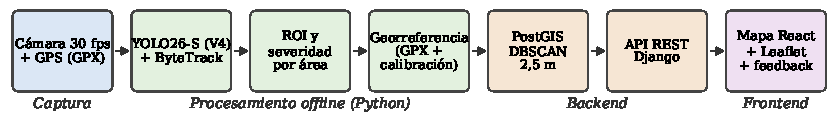
\includegraphics[width=\textwidth]{fig_pipeline.pdf}
\caption{Arquitectura de SPM: de la captura con cámara y GPS al mapa web.}
\label{fig:pipeline}
\end{figure*}

\section{Introducción y contexto}

El deterioro de la calzada es un problema persistente en las ciudades del
Paraguay. En Encarnación, la Municipalidad presentó en 2026 la plataforma
``Chau Baches'', que recibe por WhatsApp fotos y ubicaciones enviadas por los
vecinos; solo en el microcentro identificó 119 baches causados por pérdidas de
agua, de los cuales 76 seguían pendientes de reparación \cite{chaubaches2026}.
Ese relevamiento depende de que alguien envíe el aviso y no cubre de forma
sistemática la red vial. Un sistema que recorra las calles con una cámara común
y publique los baches en un mapa complementaría esos reportes y reduciría el
costo del relevamiento.

Los primeros sistemas automáticos usaron acelerómetros \cite{eriksson2008} o
procesamiento clásico de imágenes \cite{koch2011}. Con el aprendizaje profundo
dominan los detectores de una etapa de la familia YOLO \cite{redmon2016}: Maeda
\emph{et al.} \cite{maeda2018} publicaron un dataset de daños viales tomado con
teléfonos, y el desafío GRDDC \cite{arya2020} comparó soluciones en varios
países. Estos trabajos se centran en la detección por imagen; SPM completa el
ciclo con seguimiento, georreferenciación del bache, consolidación de
observaciones repetidas y validación ciudadana en un mapa web.

\section{Metodología y arquitectura del sistema}

La Fig.~\ref{fig:pipeline} resume el pipeline. El procesamiento de visión se
ejecuta \emph{offline}, sobre el video ya grabado.

\subsection{Captura y preprocesamiento}
La captura se realizó desde un automóvil: un integrante conducía y el otro, como
acompañante, operaba una laptop con el software de captura y una cámara DJI
Osmo Pocket 3, que graba video 1080p a 30\,fps con la hora UTC de cada
fotograma. En paralelo, la aplicación Open GPX Tracker 1.10.1 para iOS registró
el recorrido (un punto por segundo) en formato GPX; ambas fuentes se unen por la
hora UTC. Antes de grabar, con el vehículo detenido, se calibró la cámara sobre
el asfalto: altura de 1,35\,m, inclinación de $1{,}462^{\circ}$ y campo de visión
horizontal de $118{,}15^{\circ}$.

Para el dataset se extrajo de los videos un fotograma por segundo, más
fotogramas adicionales ante cambios grandes de escena, y se descartaron los
borrosos con un índice de nitidez. Las imágenes se etiquetaron con cajas en
Roboflow \cite{roboflow} y se redimensionan a 640\,px.

\subsection{Dataset y entrenamiento}
V3, un YOLO26 Nano con tres clases de severidad, detectó solo 32 de 64 baches
en su evaluación, pero clasificó bien 29 de esos 32 (90,6\,\%): el problema era
\emph{encontrar} baches, no clasificarlos. Por eso V4 es un detector de una sola
clase (\texttt{pothole}) y la severidad se calcula aparte. V4 usa YOLO26 Small
\cite{ultralytics} preentrenado, con 386 imágenes: 143 propias de Encarnación y
243 de un dataset público. El dataset se publicó en Roboflow Universe como
\emph{fork} del original (CC BY 4.0) \cite{dataset2026} y se dividió en 275
imágenes de entrenamiento, 74 de validación y 37 de test (70 baches). Se entrenó
hasta 300 épocas con paciencia 90; la mejor época fue la 281.

\subsection{Seguimiento, severidad y georreferenciación}
ByteTrack \cite{zhang2022} sigue cada bache entre fotogramas. Se descartan las
detecciones con centro en el 45\,\% superior de la imagen (ROI) y los
\emph{tracks} con menos de 3 fotogramas. En el fotograma de mayor área se
calcula el área normalizada con corrección de perspectiva:
\begin{equation}
A_{n} = \frac{A}{W H}\left(\frac{y_{r}-y_{h}}{\max(y-y_{h},\,d)}\right)^{\gamma},
\end{equation}
donde $A$ es el área de la caja, $W\times H$ el tamaño del fotograma, $y$ la
fila normalizada del centro, $y_h=0{,}45$, $y_r=0{,}7$, $d=0{,}05$ y
$\gamma=2$. Con la calibración del equipo, $A_n<0{,}001$ es leve,
$A_n<0{,}008$ moderado y el resto crítico. Los umbrales se calibran etiquetando
recortes en una vista interna y se aplican a la base sin reprocesar el video.

La posición del vehículo se interpola en el GPX y el rumbo se estima con
posiciones vecinas. El centro de la caja se proyecta sobre la calzada con un
modelo de cámara estenopeica y suelo plano (hasta 30\,m), de modo que se ubica
el bache y no el GPS.

\subsection{Backend, API e interfaz}
Las detecciones se importan a PostgreSQL/PostGIS, donde DBSCAN \cite{ester1996}
(radio de 2,5\,m) agrupa las observaciones de un mismo bache. Una API REST en
Django expone los baches con severidad, confianza y foto de evidencia, con
consultas por radio. El mapa web (React y Leaflet) colorea los baches por
severidad y permite reportar falsos positivos o reparaciones: cada reporte
reduce la opacidad del marcador, y con 3 falsos positivos o 1 reparación el
bache se oculta. Los conteos se guardan en el servidor, por lo que todos los
usuarios ven el mismo estado.

\section{Resultados y discusión}

\subsection{Desempeño del detector}
La Tabla~\ref{tab:modelos} compara las versiones. Para V4 se reportan el test
(Roboflow) y la validación del checkpoint; esta última es optimista porque se
usa para elegir la época. V4 supera a V3 en 21,6 puntos de mAP@50, aunque cada
uno se evaluó sobre su propio dataset.

\begin{table}[!htbp]
\caption{Métricas de las versiones del detector (\%)}
\label{tab:modelos}
\centering
\setlength{\tabcolsep}{3.2pt}
\begin{tabular}{@{}lccccc@{}}
\toprule
Modelo (fuente) & mAP@50 & mAP@50-95 & P & R & F1 \\
\midrule
V2, 1 clase & 82,7 & --- & 86,4 & 75,5 & 80,6 \\
V3, Nano, 3 clases & 39,2 & 16,9 & 63,1 & 46,2 & 53,3 \\
V4, Small, 1 clase (test) & 60,8 & 28,3 & 76,3 & 64,3 & 69,8 \\
V4, Small, 1 clase (valid.) & 69,9 & 36,7 & 88,4 & 66,1 & 75,6 \\
\bottomrule
\multicolumn{6}{@{}p{\columnwidth}@{}}{\footnotesize F1 $=2PR/(P+R)$. Cada
versión se evaluó sobre su propio dataset.}
\end{tabular}
\end{table}

La matriz de confusión de V4 en test (Tabla~\ref{tab:confusion}) muestra 45
baches detectados, 25 no detectados y 14 falsos positivos. Frente a la
validación, el recall se mantiene, pero la precisión baja 12 puntos: en imágenes
nuevas aparecen más falsos positivos, como grietas y parches.

\begin{table}[!htbp]
\caption{Matriz de confusión de V4 en test (37 imágenes)}
\label{tab:confusion}
\centering
\begin{tabular}{@{}lcc@{}}
\toprule
Real $\backslash$ Predicción & Bache & No detectado \\
\midrule
Bache & \textbf{45} & 25 \\
Fondo (falso positivo) & 14 & --- \\
\bottomrule
\end{tabular}
\end{table}

Según la Fig.~\ref{fig:map}, con la convención de tamaños de COCO
\cite{lin2014}, el modelo funciona bien con baches grandes (mAP@50 de
75,3\,\%), peor con medianos (43,2\,\%) y no detecta los chicos. Un bache lejano
se ve chico, así que solo se detecta al acercarse; el seguimiento lo compensa en
parte. La \emph{accuracy} no se reporta porque en detección de objetos no hay
verdaderos negativos contables, y el RMSE aplicaría al error de posición, que
requiere coordenadas de referencia medidas en campo.

\begin{figure}[!htbp]
\centering
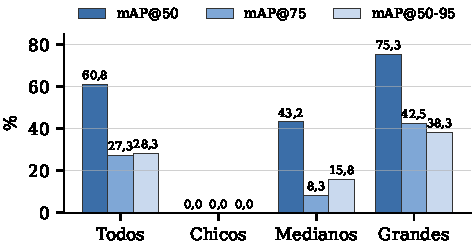
\includegraphics[width=0.85\columnwidth]{fig_map_tamano.pdf}
\caption{mAP de V4 por tamaño de objeto (evaluación de Roboflow).}
\label{fig:map}
\end{figure}

% Figura opcional (si sobra espacio): curvas de validación de V4.
% \begin{figure}[!htbp]
% \centering
% 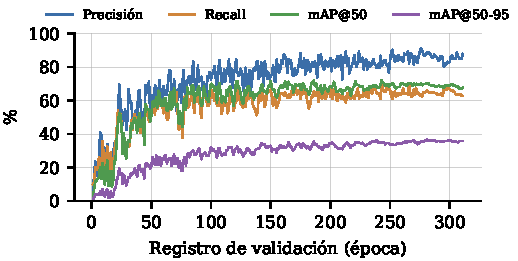
\includegraphics[width=\columnwidth]{fig_curvas_v4.pdf}
% \caption{Métricas de validación de V4 durante el entrenamiento.}
% \end{figure}

% Figura opcional (si sobra espacio): detección real con la línea de la ROI.
% \begin{figure}[!htbp]
% \centering
% 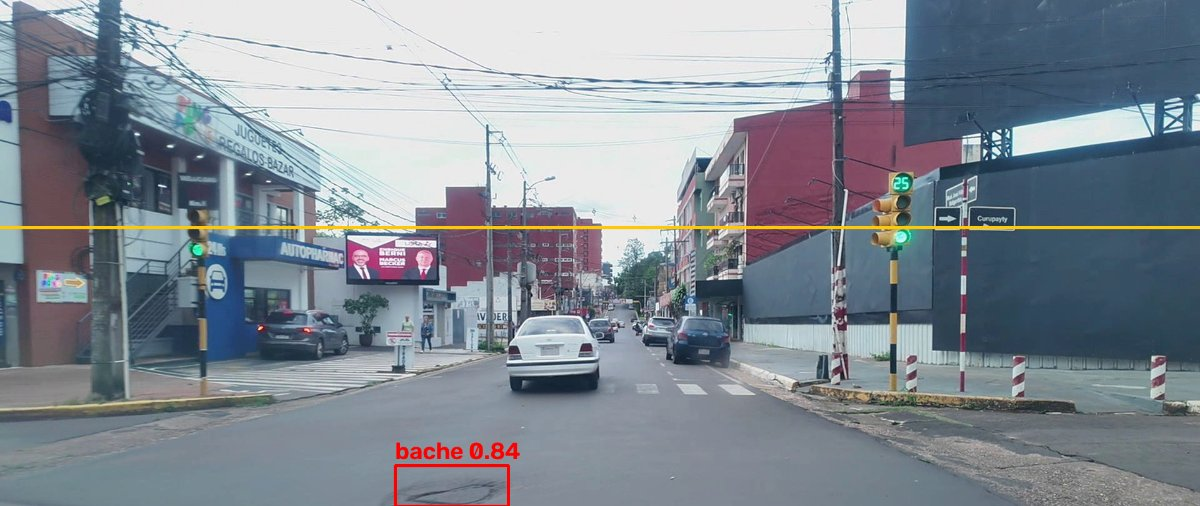
\includegraphics[width=\columnwidth]{fig_ejemplo.jpg}
% \caption{Detección en una calle de Encarnación (confianza 0,84). La línea
% horizontal marca el límite de la ROI.}
% \end{figure}

\subsection{Tiempo de inferencia y prueba de campo}
En un Intel Core i7-12700F sin GPU, V4 procesa un fotograma en 51\,ms (unos
19\,fps) con entradas de 640\,px, suficiente para el procesamiento offline; la
API en la nube de Roboflow reporta 7,5\,ms.

En la prueba de campo se procesaron 403 fotogramas de cinco recorridos del
7/11/2026 con su GPX. Hubo 117 detecciones ($\text{conf}\geq 0{,}3$), de las
cuales 115 quedaron dentro de la ROI y se georreferenciaron; DBSCAN las
consolidó en 89 baches (61 leves y 28 moderados). Ninguno resultó crítico: el
mayor $A_n$ fue 0,0049, por debajo del umbral de 0,008. La inspección visual
mostró falsos positivos en grietas y marcas pequeñas. No se reporta precisión de
campo porque esos fotogramas no tienen etiquetas y parte de ellos pudo usarse en
el entrenamiento.

\section{Conclusiones y trabajo futuro}

SPM demuestra que un pipeline de bajo costo, con una cámara común, el GPS de un
teléfono y un detector que corre en CPU, puede relevar baches y publicarlos en
un mapa georreferenciado. La lección principal fue separar la detección de la
severidad: un detector de una clase superó al modelo de tres clases, y la
severidad pasó a ser una regla geométrica configurable y explicable.

Como limitaciones, el modelo no detecta baches chicos o lejanos; con un recall
de 64,3\,\% deja pasar uno de cada tres, y su precisión de 76,3\,\% implica
que uno de cada cuatro avisos es falso, algo que el feedback ciudadano ayuda a
depurar. El dataset es pequeño y no se midió el error de georreferenciación.
Como trabajo futuro se propone ampliar el dataset con recorridos propios
separados entre entrenamiento y test, entrenar con mayor resolución para los
baches chicos, refinar los umbrales de severidad, medir el error de posición
(RMSE) en campo y usar el feedback ciudadano para reentrenar el modelo.

\begin{thebibliography}{00}
\bibitem{chaubaches2026} Edición Prensa, ``Municipalidad presenta `Chau Baches' para reportar daños en la vía pública,'' \emph{Más Encarnación}, Encarnación, Paraguay, 7 jul. 2026. [En línea]. Disponible: \url{https://www.masencarnacion.com/articulo/municipalidad-presenta-chau-baches-para-reportar-danos-en-la-publica} [Accedido: 9 nov. 2026].
\bibitem{eriksson2008} J. Eriksson, L. Girod, B. Hull, R. Newton, S. Madden y H. Balakrishnan, ``The Pothole Patrol: Using a mobile sensor network for road surface monitoring,'' en \emph{Proc. 6th Int. Conf. Mobile Systems, Applications, and Services (MobiSys)}, 2008, pp. 29--39.
\bibitem{koch2011} C. Koch e I. Brilakis, ``Pothole detection in asphalt pavement images,'' \emph{Advanced Engineering Informatics}, vol. 25, no. 3, pp. 507--515, 2011.
\bibitem{redmon2016} J. Redmon, S. Divvala, R. Girshick y A. Farhadi, ``You only look once: Unified, real-time object detection,'' en \emph{Proc. IEEE Conf. Computer Vision and Pattern Recognition (CVPR)}, 2016, pp. 779--788.
\bibitem{maeda2018} H. Maeda, Y. Sekimoto, T. Seto, T. Kashiyama y H. Omata, ``Road damage detection and classification using deep neural networks with smartphone images,'' \emph{Computer-Aided Civil and Infrastructure Engineering}, vol. 33, no. 12, pp. 1127--1141, 2018.
\bibitem{arya2020} D. Arya \emph{et al.}, ``Global road damage detection: State-of-the-art solutions,'' en \emph{Proc. IEEE Int. Conf. Big Data}, 2020, pp. 5533--5539.
\bibitem{ultralytics} Ultralytics, ``Ultralytics YOLO,'' 2026. [En línea]. Disponible: \url{https://docs.ultralytics.com}
\bibitem{roboflow} Roboflow, Inc., ``Roboflow,'' 2026. [En línea]. Disponible: \url{https://roboflow.com}
\bibitem{dataset2026} New Workspace, ``pothole Dataset,'' Roboflow Universe, nov. 2026. Licencia CC BY 4.0. [En línea]. Disponible: \url{https://universe.roboflow.com/lucas-benitez/pothole-vhmow-bygvr} [Accedido: 9 nov. 2026].
\bibitem{zhang2022} Y. Zhang \emph{et al.}, ``ByteTrack: Multi-object tracking by associating every detection box,'' en \emph{Proc. European Conf. Computer Vision (ECCV)}, 2022, pp. 1--21.
\bibitem{ester1996} M. Ester, H.-P. Kriegel, J. Sander y X. Xu, ``A density-based algorithm for discovering clusters in large spatial databases with noise,'' en \emph{Proc. 2nd Int. Conf. Knowledge Discovery and Data Mining (KDD)}, 1996, pp. 226--231.
\bibitem{lin2014} T.-Y. Lin \emph{et al.}, ``Microsoft COCO: Common objects in context,'' en \emph{Proc. European Conf. Computer Vision (ECCV)}, 2014, pp. 740--755.
\end{thebibliography}

\end{document}
